\documentclass[]{report}

\usepackage[portuguese]{babel}
\usepackage[utf8]{inputenc}
\usepackage{graphicx}
\usepackage{hyperref}
\usepackage{mdwlist}
\usepackage{pslatex}
\usepackage{makeidx}
\usepackage{textcomp}
\usepackage{float}
% Title Page
\title{}
\author{Renan Birck Pinheiro}

\makeindex
\begin{document}
\begin{titlepage}
\begin{center}

\textsc{\LARGE Universidade Federal de Santa Maria}\\[1.5cm]
\textsc{\Large Centro de Tecnologia}\\[0.5cm]
\textsc{\Large Departamento de Eletrônica e Computação}\\[0.5cm]
\textsc{\Large Disciplina: Princípios de Telecomunicações}\\[0.5cm]
\setlength{\oddsidemargin}{0pt} % Tirar as margens gigantes que o LaTeX põe
\setlength{\evensidemargin}{0pt} % evitar desperdício de papel
\setlength{\textwidth}{15cm}
\end{center}

\vspace*{5cm}
\begin{center}
{\huge \bfseries Estudo sobre Modulação de Sinais}\\[0.4cm]
\end{center}

\vspace*{130px}
\begin{flushright}
\emph{Autores:}
Caio S. Guedes $<$\url{caio_ee@hotmail.com}$>$ \newline
Marcelo Brum $<$\url{marcelobrum.rs@gmail.com}$>$ \newline
Renan Pinheiro $<$\url{renan.ee.ufsm@gmail.com}$>$. \newline



\end{flushright}
\begin{center}
Santa Maria, \today.

\end{center}


\end{titlepage}
\tableofcontents

\chapter{Introdução}
Neste trabalho serão abordadas as práticas feitas em laboratório, na discplina de Princípios de Telecomunicações, visando estudar o funcionamento das modulações em amplitude (AM) e em frequência (FM). Também será abordada a modulação por códigos de pulso (PCM). 

\chapter{Experimento 1: Modulação AM a diodo}
\section{Fundamentação Teórica}
Seja um sinal senoidal modulante dado por 

\begin{equation}\label{eq_modulante}
V_s = A \cos(\omega_s t + \phi)
\end{equation}

e uma portadora dada por

\begin{equation}\label{eq_portadora}
V_p = A \cos(\omega_p t + \phi)
\end{equation}

tal que $\omega_p > \omega_s$. A fase dos sinais é fixa em 0, assim eliminando-se $\phi$. Para a análise no domínio da frequência, reescrevem-se os cossenos na forma exponencial e usam-se as propriedades de Fourier.

A modulação em amplitude (\textit{Amplitude Modulation}) feita desta forma resulta em duas \textit{sidebands}, posicionadas em $F_s$ \textpm $F_c$.

Problema proposto:
\begin{quote}
Implemente o circuito da Figura 1 e calcule a frequência de ressonância do filtro passa faixa. Ajuste a freqüência de $E_o(t)$ para o valor calculado. Ajuste a freqüência de $a(t)$ para 1KHz. Faça a amplitude de $E_0(t)$ igual a 10V pico a pico e a de $a(t)$ 3V pico a pico. Apresente suas conclusões a respeito do uso do filtro e da freqüência de ressonância obtida.
\end{quote}

\section{Procedimento experimental}
O circuito da figura \ref{fig:demodulador_AM_diodo} foi montado em uma \textit{protoboard}:
\begin{figure}[H]
\centering 
\begin{center}
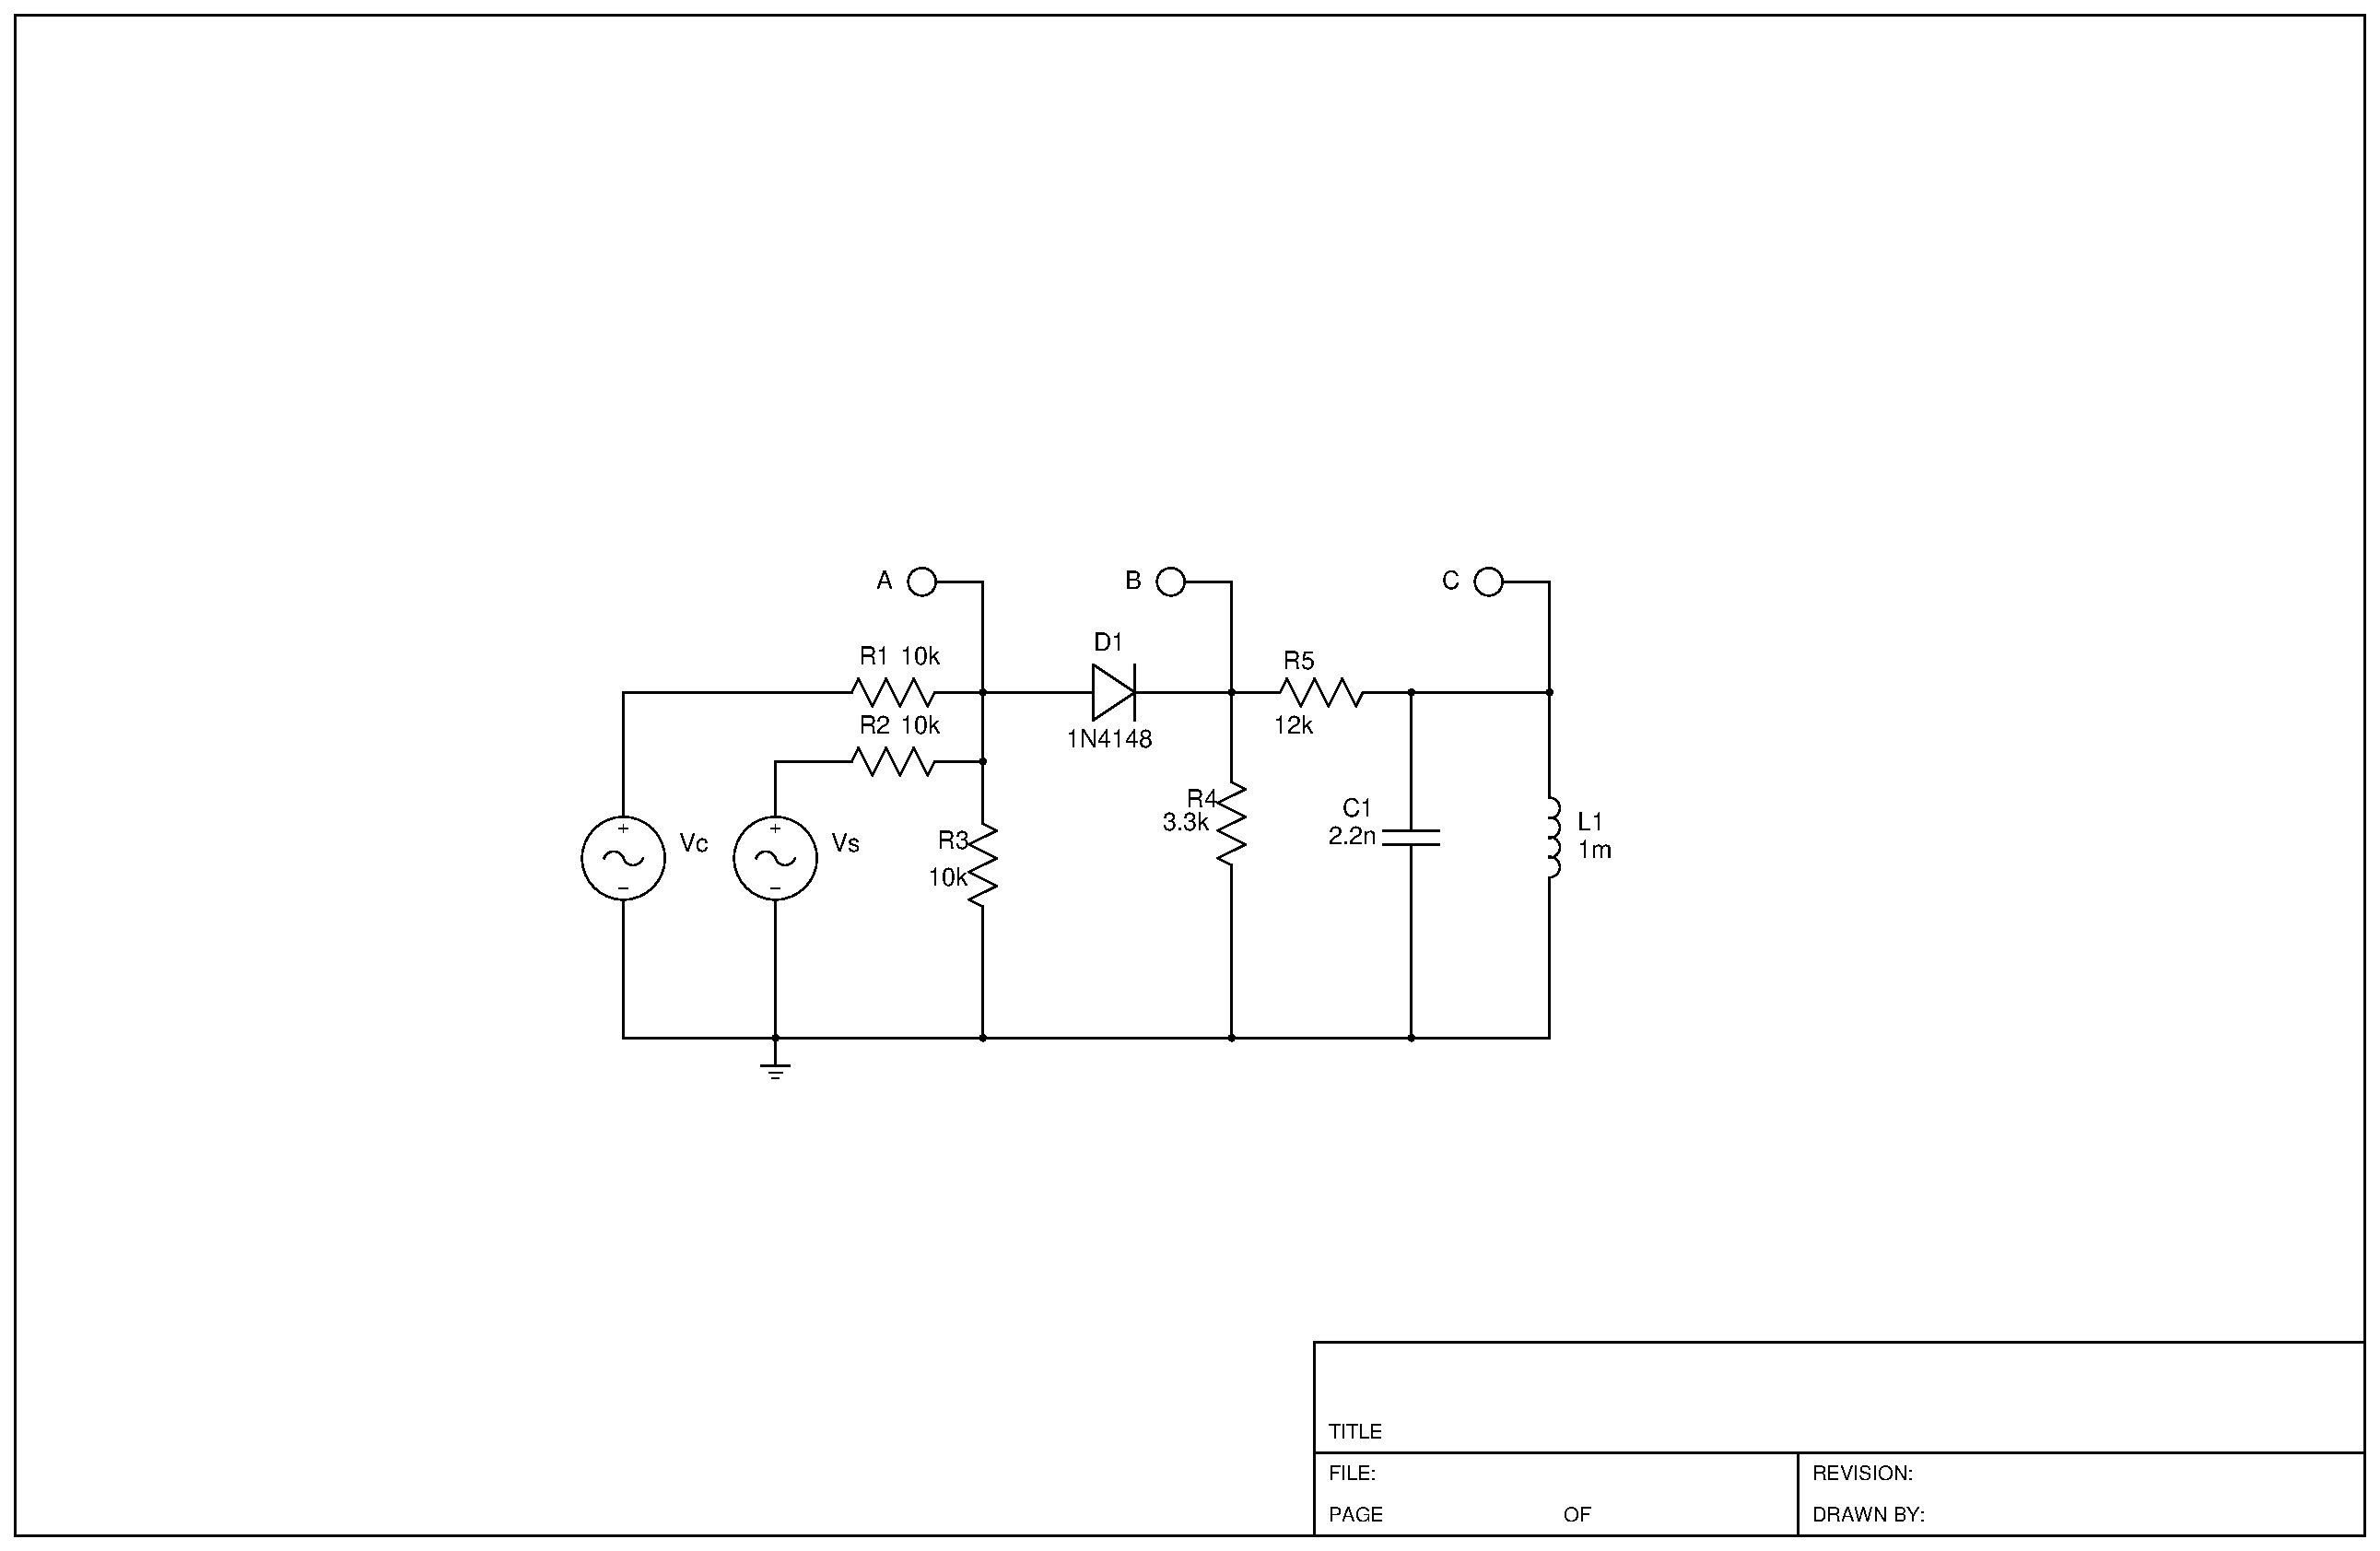
\includegraphics[scale=0.4,clip]{./imagens/AM_Modulator_Diode}
\end{center}
\caption{Modulador AM a diodo.}
\label{fig:demodulador_AM_diodo}
\end{figure}

Para sintonizar a portadora, calcula-se a frequência de ressonância do filtro LC da saída:

\begin{equation}
f_0 = \frac{1}{2 \pi \sqrt{LC}}
\end{equation}

Para os valores fornecidos ($C = 2,2 nF$ e $L = 1000 \mu F$) ter-se-á que essa frequência será de cerca de 107 KHz. 

Após sintonizados os sinais de portadora e da modulante, mede-se a saída.

\chapter{Experimento 2: Modulação AM a transistor}
\section{Introdução}
\chapter{Experimento 3: Transmissão e recepção de FM}
\section{Demodulação FM}
Ela também pode ser feita utilizando-se um circuito PLL (\textit{Phase-Locked Loop}), o qual foge do foco do presente trabalho.
\chapter{Experimento 4: Modulação por código de pulso (PCM)}
\section{Introdução}
PCM é uma técnica para a representação de sinais analógicos convertidos para formato digital, visando transmissão ou posterior processamento. Uma codificação em PCM transforma uma amostra quantizada em um número codificado. \cite{renatodatacom}

Fundamentalmente, a técnica consiste na quantização dos dados através de um conversor A/D. No lado do receptor existirá um conversor D/A que irá fazer o processo oposto.

\bibliographystyle{alpha}
\begin{thebibliography}{100}
\bibitem{renatodatacom}
 MACHADO, R. 
 \textbf{Notas de aula da disciplina de Comunicação de Dados.}
 Disponível em \url{http://www.ufsm.br/gpscom/professores/Renato\%20Machado/comunicacaodedados.html}. Acessado em 12/06/2012.
 
\bibitem{wolframeuler}
 \textbf{Euler Formula}. Disponível em \url{http://mathworld.wolfram.com/EulerFormula.html}. Acessado em 23/06/2012.
\end{thebibliography}
\end{document}          
